\documentclass[a4paper,14pt]{article}
\usepackage{float}
\usepackage{extsizes}
\usepackage{amsmath}
\usepackage{amssymb}
\everymath{\displaystyle}
\usepackage{geometry}
\usepackage{fancyhdr}
\usepackage{multicol}
\usepackage{graphicx}
\usepackage[brazil]{babel}
\usepackage[shortlabels]{enumitem}
\usepackage{cancel}
\usepackage{textcomp}
\usepackage{array} % Para melhor formatação de tabelas
\usepackage{longtable}
\usepackage{booktabs}  % Para linhas horizontais mais bonitas
\usepackage{float}   % Para usar o modificador [H]
\usepackage{caption} % Para usar legendas em tabelas

\columnsep=2cm
\hoffset=0cm
\textwidth=8cm
\setlength{\columnseprule}{.1pt}
\setlength{\columnsep}{2cm}
\renewcommand{\headrulewidth}{0pt}
\geometry{top=1in, bottom=1in, left=0.7in, right=0.5in}

\pagestyle{fancy}
\fancyhf{}
\fancyfoot[C]{\thepage}

\begin{document}
	
	\noindent\textbf{6FMA91 - Matemática} 
	
	\begin{center}Revisão: introdução aos conjuntos, diagrama de Venn, intersecção e união (Versão estudante)
	\end{center}
	
	\noindent\textbf{Nome:} \underline{\hspace{10cm}}
	\noindent\textbf{Data:} \underline{\hspace{4cm}}
	
	%\section*{Questões de Matemática}
	~ \\ ~
	\begin{multicols}{2}
	\noindent Fatos importantes que você precisa lembrar: \\
	1. Tabela-verdade: \\
	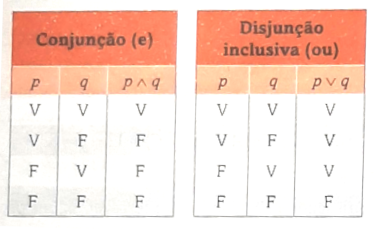
\includegraphics[width=1\linewidth]{imagens_6FMA91/imagem1}
	2. União e intersecção: \\
	$A \cup B = {x \in U : x \in A \lor x \in B}$ \\
	$A \cap B = {x \in U : x \in A \land x \in B}$ \\
	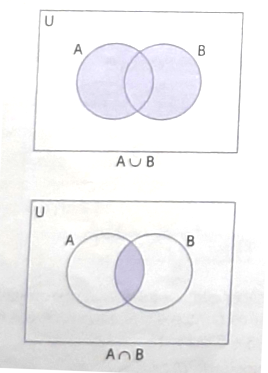
\includegraphics[width=0.7\linewidth]{imagens_6FMA91/imagem2} \\
	\noindent\textsubscript{~--------------------------------------------------------------------------}	
    	\begin{enumerate}
    		\item $A = \{2, 3, 4\}, B = \{3, 4, 5, 6\}$ e $C = \{2, 4, 6, 8\}$. Apresentar:
    		\begin{enumerate}[a)]
    			\item $A \cap B$ 
    			\item $A \cap B \cap C$ \\\\\\\\\\\\
    			\item $A \cup C$ \\\\\\\\\\\\
    			\item $(A \cup B) \cap C$ \\\\\\\\\\\\
    		\end{enumerate}
    		\item Hachurar:
    		\begin{enumerate}[a)]
    			\item $(A \cup B) \cap C$ \\
    			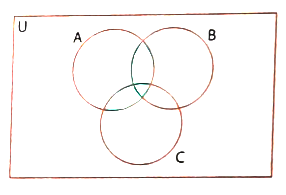
\includegraphics[width=1\linewidth]{imagens_6FMA91/imagem3}
    			\item $(C \cap B) \cup A$ \\
    			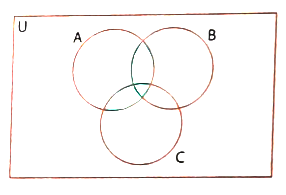
\includegraphics[width=1\linewidth]{imagens_6FMA91/imagem3}
    			\item $B \cup (A \cap C)$ \\
    			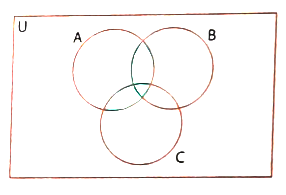
\includegraphics[width=1\linewidth]{imagens_6FMA91/imagem3}
    		\end{enumerate}
    		\item Assinale \textbf{V} (verdadeiro) ou \textbf{F} (falso).
    		\begin{enumerate}[a)]
    			\item (~~) 5 é primo $\land$ 7 é ímpar.
    			\item (~~) 18 - 7 = 11 e 28 : 4 = 5.
    			\item (~~) $\frac{8}{9} = \frac{2}{3} \lor 42 + 19 = 62$.
    			\item (~~) 47 + 13 = 50 ou 10 é múltiplo de 2.
    		\end{enumerate}
    		\item Dados os conjuntos $A = \{1, 2\}, B = \{2, 3\} e C = \{ 0, 3, 5\}$, determine:
    		\begin{enumerate}[a)]
    			\item $A \cup B$
    			\item $A \cap B$
    			\item $A \cup C$
    			\item $A \cap C$
    			\item $(A \cap B) \cup C$
    			\item $A \cap (B \cup C)$
    			\item $(A \cup B) \cap (A \cup C)$\\\\
    		\end{enumerate}
    		\item Apresente os conjuntos listando os seus elementos.
    		\begin{enumerate}[a)]
    			\item $A = \{x \in N : x~$é múltiplo de 15\}
    			\item $B = \{x \in N : x~$é menor que 7\}
    			\item $C = \{x \in N : x~$é primo e par\}
    		\end{enumerate}
    	\end{enumerate}
    $~$ \\ $~$ \\ $~$ \\ $~$ \\ $~$ \\ $~$ \\ $~$ \\ $~$ \\ $~$ \\ $~$ \\ $~$ \\ $~$ \\ $~$ \\ $~$ \\ $~$ \\ $~$ \\ $~$ \\ $~$ \\ $~$ \\ $~$ \\ $~$ \\ $~$ \\ $~$ \\ $~$ \\ $~$ \\ $~$ \\ $~$ \\ $~$ \\ $~$ \\ $~$ \\
	\end{multicols}
\end{document}